\documentclass[11pt,a4paper,oneside]{article}

%\usepackage{pscyr}
\usepackage[T2A]{fontenc}
\usepackage[utf8x]{inputenc}
\usepackage[english,russian]{babel}
\usepackage{expdlist}
\usepackage[dvips]{graphicx}
\usepackage{subcaption}
\usepackage{amsmath}
\usepackage[makeroom]{cancel}
\usepackage{svg}
\usepackage[top=1in, bottom=1in, left=1in, right=1in]{geometry}
\usepackage{indentfirst}
\usepackage{mathtools}

\begin{document}

\begin{center}
	{Вяцков Михаил, КН-401}
	
	{\huge \bf Лабораторная работа №4}
\end{center}

\section{Условия}

Необходимо посчитать различными методами приближенное значение интеграла

$$ \int\displaylimits_{a}^{b} f(x) dx
	= \int\displaylimits_{0.3}^{1.1} \ln \left( \arctan(x) \right) dx $$

Функция логарифма является аналитической на интересующем нас отрезке, как и функция арктангенса, а значит их композиция тоже аналитическая, значит $f(x)$ дифференцируема бесконечное число раз.

Пусть в очередном методе происходит разбиение отрезка на $n$ частей. Положим заранее для удобства

$$ \frac{b - a}{n} = h $$
$$ I[f] = \int_{a}^{b} f(x) dx $$
$$ M_k(f) = \max_{x \in [a, b]} \left| f^{(k)}(x) \right| $$

Для дальнешего использования найдем также явно первую производную подынтегральной функции

$$ f'(x) = \frac{1}{arctan(x)} \frac{1}{1 + x^2} $$

\section{Методы}

\subsection{Метод средних прямоугольников}

Метод средних прямоугольников является интерполяционной формулой численного интегрирования степени $0$ на отрезке $[a, b]$ с узлом в $\frac{a + b}{2}$. Это дает нам следующее выражение для приближенного значения интеграла

$$ S_1[f] = A_0 f \left( \frac{a + b}{2} \right) $$

Так как алгебраическая точность не меньше степень интерполяционного многочлена, то формула точна для полиномов степени $0$, например $f(x) \equiv 1$

$$ S_1[f \equiv 1] = A_0 \cdot 1 = \int_{a}^{b} f(x) dx = b - a $$
$$ A_0 = b - a $$

Отсюда получаем формулу

$$ S_1[f] = (b - a) f \left( \frac{a + b}{2} \right) $$

Используя такое выражение, построим составную формулу интегрирования

$$ S_1^n[f] = \sum_{i = 0}^{n - 1} h f \left( a + \left( i + \frac{1}{2} \right) h \right) $$

Погрешность элементарной версии данной формулы можно построить следующим образом. Заметим, что алгебраическая точность формулы средних прямоугольников составляет $n_{\alpha} = 1$, проверить это можно в лоб, подставив $f(x) = 1; x; x^2$. Теперь воспользуемся тем, что из-за этого многочлен Эрмита $H[f]$, построенный по двум одинаковым узлам в $\frac{a + b}{2}$, имеющий степень $1$, будучи приближенно вычисленным с помощью данного метода, даст точное значение. Таким образом

$$ E_1[f] = I[f] - S_1[f] = I[f] - S_1[H(f)] = I[f] - I[H(f)] = I[f - H(f)] = I[R_H(f)] $$

Воспользовавшись тем, что

$$ R_H(f) = f \left( x, \frac{a + b}{2}, \frac{a + b}{2} \right) \left( x - \frac{a + b}{2} \right)^2 $$

и первой теоремой о среднем (т.к. второй множитель неотрицателен), получаем

$$ \int_{a}^{b} f \left( x, \frac{a + b}{2}, \frac{a + b}{2} \right) \left( x - \frac{a + b}{2} \right)^2 dx
	= f \left( \xi, \frac{a + b}{2}, \frac{a + b}{2} \right) \int_{a}^{b} \left( x - \frac{a + b}{2} \right)^2 dx
	=  $$
$$ = f \left( \xi, \frac{a + b}{2}, \frac{a + b}{2} \right) \frac{(b - a)^3}{12}
	= \frac{f''(\mu)}{2} \frac{(b - a)^3}{12} = f''(\mu) \frac{(b - a)^3}{24} $$
$$ \xi, \mu \in [a, b] $$

Таким образом погрешность элементарной формулы средних прямоугольников

$$ \left| E_1[f] \right| \le M_2(f) \frac{(b - a)^3}{24} $$

В случае составной формулы мы складываем $n$ слагаемых с определенной выше погрешностью, получая в итоге

$$ \left| E_1^n[f] \right| \le n \left| E_1[f] \right| = M_2(f) (b - a) \frac{h^2}{24} $$

\subsection{Метод Эйлера}

Пусть задан отрзок $[a, b]$ и дифференцируемая на этом отрезке функция $f(x)$. Построим интерполяционий многочлен Эрмита по узлам $x_0 = a, x_1 = b$, каждый узел взяв два раза и используя значения $f(x_0), f'(x_0), f(x_1), f'(x_1)$ соотвественно. Тогда проинтегрировав этот многочлен, получим формулу.

$$ S_2[f] = A_0 f(x_0) + A_1 f'(x_0) + B_0 f(x_1) + B_1 f'(x_1) $$

Используя то, что алгебраическая степень интерполяционной формулы не ниже степени интерполяции, получим, что алгебраическая степень данной формулы не ниже третей, то есть формулы точна для всех полиномов такой степени.

Подставляя в фомулу многочлены $f(x) \equiv 1; f(x) = x - \frac{a + b}{2}; f(x) = \left( x - \frac{a + b}{2} \right)^2; f(x) = \left( x - \frac{a + b}{2} \right)^3$ можно получить следующее выражение для коэффицентов

$$ S_2[f] = \frac{b - a}{2} \left( f(a) + f(b) \right) + \frac{(b - a)^2}{12} \left( f'(a) - f'(b) \right) $$

Эта формула и называется формулой Эйлера.

Так как это интерполяционная формула, то погрешность вычисляется стандартно

$$ E_2[f] = I[R_2[f]] = \int_{a}^{b} f (x, a, a, b, b) (x - a)^2 (x - b)^2 dx $$

Используя теорему о среднем и выражение для разделенной разности через производную

$$ E_2[f] = \frac{f^{(4)}(\xi)}{4!} \int_{a}^{b} (x - a)^2 (x - b)^2 dx
	= \frac{f^{(4)}(\xi)}{4!} \frac{(b - a)^5}{30} $$
$$ \left| E_2[f] \right| \le \frac{M_4(f) (b - a)^5}{720} $$

Составная формула таким образом выглядит так

$$ S_2^n = \frac{h}{2} \left( 2 \left( \sum_{i = 0}^{n} f(a + ih) \right) - f(a) - f(b) \right) + \frac{h^2}{12} (f'(a) - f'(b)) $$

И ее погрешность, конечно же оценивается как

$$ \left| E_2^n[f] \right| \le \frac{M_4(f) (b - a) h^4}{720} $$


\subsection{Погрешность по Рунге}

Часто возникает необходимость без оценок сложновычислимых производных посчитать погрешность вычисления интеграла при некотором уточняющем процессе. Пусть в таком случае мы применяем составной метод интегрирования, который зависит от параметра $h$, расстояния, на котором отстоят друг от друга точки. Тогда исходной интеграл можно представить в виде

$$ I[f] = S[f](h) + E[f](h) $$

Пусть также погрешность вычисления обладает следующей ассимптотикой

$$ R[f](h) = C h^p + o(h^p) $$

Тогда составим систему уравнений для двух значений параметра~--- $h$ и $h / 2$

$$ \left\{ \begin{array}{l}
	I[f] = S[f](h) + E[f](h) \\
	I[f] = S[f](h / 2) + E[f](h / 2)
\end{array} \right. $$

Заметим, что в силу ассимптотического разложение погрешности

$$ E[f](h) = C h^p + o(h^p) = 2^{p} (C (h / 2)^p + o(h^p) \approx 2^{p} E[f](h / 2) $$

Знак примерного равенства происходит из того, что когда мы пишем знак равенства вместе с о-маленьким, на самом деле это означает включение в класс множеств.

Исключив истинное значение интеграла, получаем соотношение

$$ E[f](h) (1 - 2^{-p}) \approx S[f](h / 2) - S[f](h) $$
$$ E[f](h) \approx \frac{S[f](h / 2) - S[f](h)}{1 - 2^{-p}}
	= \frac{2^p \left( S[f](h / 2) - S[f](h) \right)}{2^p - 1} $$

В контексте решаемой задачи, рассмотрим погрешности каждого из составных методов. Для этого заметим, что любой интерполяционный метод численного интегрирования степени 0 дает при определении коэффицентов формулу

$$ S_3[f] = (b - a) f(\xi), \xi \in [a, b] $$

И обладает погрешностью второго порядка малости относительно длины отрезка, на котором производится интегрирование, это можно показать, воспользовавшись формулой о среднем для интеграла и затем теоремой Лагранжа о среднем значении

$$ \left| E_3[f] \right| = \left| I[f] - S_3[f] \right|
	= \left| f(\mu) (b - a) - f(\xi) (b - a) \right|
	= \left| f'(\zeta) (b - a)^2 \right| \le M_1(f) (b - a)^2 $$

Из этого следует, что можно сделать следующие умозаключения

$$ \sum_{i = 0}^{n - 1} g(\mu_i) h = \sum_{i = 0}^{n - 1} \int_{a + ih}^{a + (i + 1)h} g(x) dx + O(h^2)
	= \int_{a}^{b} g(x) dx + O(h) $$
	
В приложении к расчету разложений для методов, рассмотренных выше и воспользовавшись тем, что $h \to 0$, получаем

$$ E_1[f](h) = \frac{h^2}{24} \sum_{i = 0}^{n - 1} f''(\xi_i) h
	= \frac{h^2}{24} \int_{a}^{b} f''(x) dx + O(h^3) = C h^2 + o(h^2) $$
$$ E_2[f](h) = h^4 \sum_{i = 0}^{n - 1} \frac{f^{(4)}(\xi)}{720} h = C h^4 + o(h^4) $$

Таким образом для метода средних прямоугольников

$$ E_1[f](h) \approx \frac{4 \left( S[f](h / 2) - S[f](h) \right)}{3} $$

А для метода Эйлера

$$ E_2[f](h) \approx \frac{16 \left( S[f](h / 2) - S[f](h) \right)}{15} $$

\subsection{Метод Гаусса с 3 узлами}

Сделаем замену переменной

$$ x = 0.4 u + 0.7 $$
$$ \int\displaylimits_{0.3}^{1.1} \ln \left( \arctan(x) \right) dx
	= \int\displaylimits_{-1}^{1} 0.4 \ln \left( \arctan(0.4 u + 0.7) \right) du $$
	
Воспользуемся методом Гаусса. Для этого нам надо построить формулу наивысшей алгебраической точности. Для этого надо решить следующую систему, доказывается, что в результате решения этой системы мы получаем коээфиценты многочлена, который имеет 3 вещественных корня на отрезке $[-1, 1]$, и таким образом эти корни образуют узлы разбиения для построения формулы численного интегрирования наивысшей алгебраической точности.

$$
\left\{ \begin{array}{l}
	\int_{-1}^{1} (x^3 + a_2 x^2 + a_1 x + a_0) dx = 0 \\
	\int_{-1}^{1} (x^3 + a_2 x^2 + a_1 x + a_0) x dx = 0 \\
	\int_{-1}^{1} (x^3 + a_2 x^2 + a_1 x + a_0) x^2 dx = 0 \\
\end{array} \right.
$$

$$
\left\{ \begin{array}{l}
	\frac{2}{3} a_2 + 2 a_0 = 0 \\
	\frac{2}{5} + \frac{2}{3} a_1 = 0 \\
	\frac{2}{5} a_2 + \frac{2}{3} a_0 = 0 \\
\end{array} \right.
$$

$$
\left\{ \begin{array}{l}
	a_2 + 3 a_0 = 0 \\
	3 + 5 a_1 = 0 \\
	3 a_2 + 5 a_0 = 0 \\
\end{array} \right.
$$

Решение этой системы уравнений очевидным образом приводит нас к многочлену

$$ Q(x) = x^3 - \frac{3}{5} x $$

Корни которого находятся в точках

$$ x_1 = 0; x_{0, 2} = \pm \sqrt{\frac{3}{5}} $$

Теперь методом неопределенных коээфицентов определим квадратурную формулу

$$ S_G[f] = A_0 f \left( -\sqrt{\frac{3}{5}} \right) + A_1 f(0) + A_2 f \left(\sqrt{\frac{3}{5}} \right) $$


$$
\left\{ \begin{array}{l}
	S_G[f \equiv 1] = A_0 + A_1 + A_2 = 2 \\
	S_G[f = x] = -\sqrt{\frac{3}{5}} A_0 + \sqrt{\frac{3}{5}} A_2 = 0 \\
	S_G[f = x^2] = \frac{3}{5} A_0 + \frac{3}{5} A_2 = \frac{2}{3} \\
\end{array} \right.
$$

Отсюда получаем итоговую формулу

$$ S_G[f] = \frac{5}{9} f \left( -\sqrt{\frac{3}{5}} \right) + \frac{8}{9} f(0) + \frac{5}{9} f \left(\sqrt{\frac{3}{5}} \right) $$

Эта формула имеет наибольшую алгебраическую точность 5 среди всех методов, использующих 3 узла.

\section{Численный эксперимент}

\begin{tabular}{| c | c | c | c | c |}
	\hline
	Метод        & $h$   & $S[f]$        & По Рунге        & $| E[f] |$ \\ \hline \hline
	Ср. Прямоуг. & 0.1   & -0.4621275855 & 0.0085097603    & 0.0145825855 \\ \cline{2-5}
	             & 0.05  & -0.4557452653 & 0.0051567845    & 0.0082002653 \\ \cline{2-5}
                 & 0.025 & -0.4518776769 & 0.0028100841    & 0.0043326769 \\ \hline
    Эйлера       & 0.1   & -0.4475351536 & 0.0000098339    & 0.0000098464 \\ \cline{2-5}
                 & 0.05  & -0.4475443728 & 0.0000006292    & 0.0000006272 \\ \cline{2-5}
                 & 0.025 & -0.4475449627 & 0.0000000396    & 0.0000000373 \\ \hline
    Гаусса       &       & -0.4473764506 &                 & 0.0001685494 \\ \hline
\end{tabular}

\section{Выводы}

\subsection{Точность}

Из приведенных выкладок можно сделать вывод, что наиболее точным методом среди рассмотренных является метод Эйлера.

Несмотря на то, что метод Гаусса обладает большей алгебраической точностью, он дает бОльшую ошибку из-за того, что использует только 3 узла, тогда как метод Эйлера с шагом 0.1 уже использует почти в 3 раза больше узлов (и еще в два раза, если считать значения производных).

Метод средних треугольников ожидаемо показал наименьшую точность, так как в целом небольшой точностью из-за того, что использует только один узел на каждом шаге.

\subsection{Изменение погрешности}

\begin{figure}
	\begin{subfigure}{\textwidth}
		\centering
		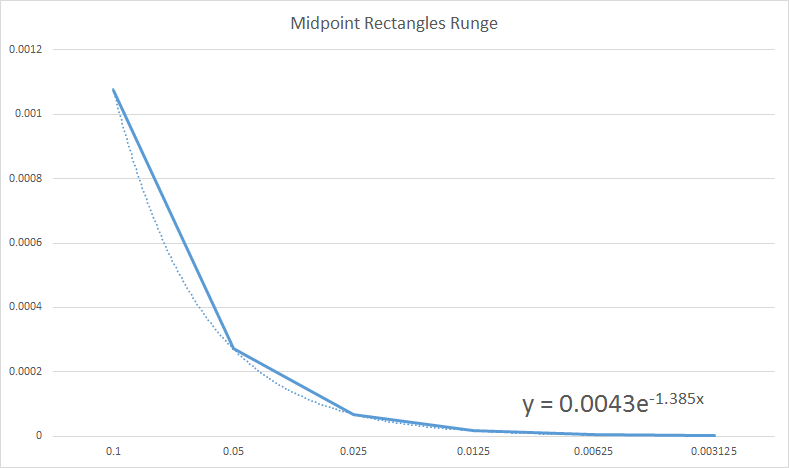
\includegraphics[width=0.8\linewidth]{pics/midpoint_errors.png}
		\caption{Изменение погрешности в методе средних треугольников}
	\end{subfigure}
	\begin{subfigure}{\textwidth}
		\centering
		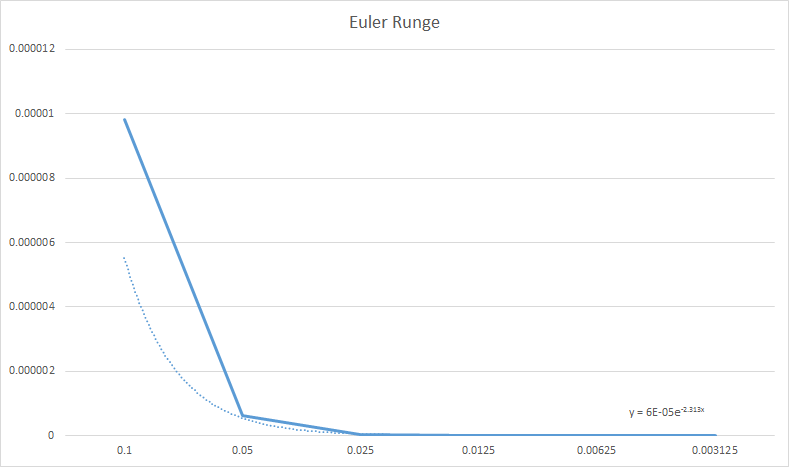
\includegraphics[width=0.8\linewidth]{pics/euler_errors.png}
		\caption{Изменение погрешности в методе Эйлера}
	\end{subfigure}
\end{figure}

Добавив еще несколько итераций для наглядности, можно заметить, что реальных данные неплохо укладываются в теорию, линия тренда у метода средних прямоугольников имеет экспоненту $e^{-0.642} = 0.526 \approx 0.5$, а линия трнда у метода Эйлера $e^{-2.496} = 0.0824 \approx 0.0625$, что согласуется с 1 порядком роста ошибки у метода средних прямоугольников и 4 порядком роста у метода Эйлера.

\end{document}
